\begin{exercice*}[Diagrammes]
    Dans une classe de $24$ élèves, il y a $16$ filles.
    \begin{enumerate}
        \item L'un des diagrammes suivants peut-il représenter correctement
        la répartition des élèves de la classe ?

        \medskip
        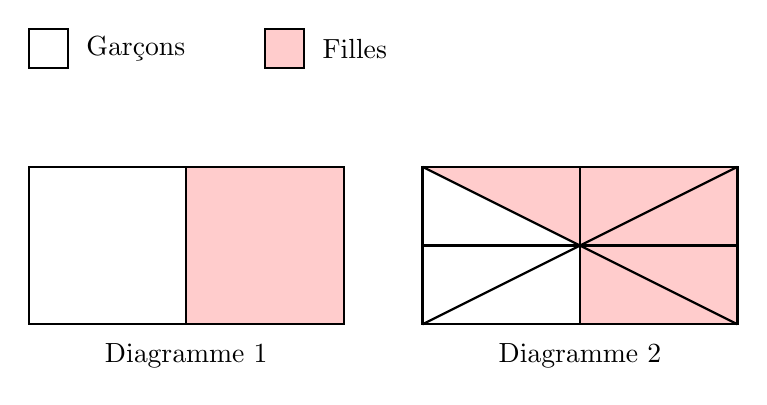
\begin{tikzpicture}
            % \draw[help lines, color=gray!30, dashed] (0,0) grid (9,5);
            \draw[thick] (0,4.25) rectangle ++(0.5,0.5);        
            \draw[shift={(0.6,4.5)},thick] node[right,fill=white] {Garçons};
            \draw[thick,fill=red!20] (3,4.25) rectangle ++(0.5,0.5);        
            \draw[shift={(3.6,4.5)},thick] node[right,fill=white] {Filles};
            \fill[color=red!20] (2,1)--(2,3)--(4,3)--(4,1)--cycle;
            \draw[thick] (0,1) rectangle ++(4,2);        
            \draw[-,thick] (2,1)--(2,3);                    
            \draw[shift={(2,0.6)},thick] node[midway,fill=white] {Diagramme 1};
            \fill[color=red!20] (5,3)--(9,3)--(9,1)--(7,1)--(7,2)--cycle;
            \draw[thick] (5,1) rectangle ++(4,2);            
            \draw[-, thick] (7,1)--(7,3);
            \draw[-, thick] (5,2)--(9,2);
            \draw[-, thick] (5,1)--(9,3);
            \draw[-, thick] (5,3)--(9,1);
            \draw[shift={(7,0.6)},color=black,ultra thick] node[midway,fill=white] {Diagramme 2};
        \end{tikzpicture}
        \item On a représenté la répartition des élèves de cette classe par un diagramme circulaire.

        \medskip
        \begin{minipage}{0.16\textwidth}
        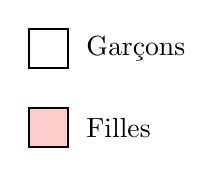
\begin{tikzpicture}
            % \draw[help lines, color=gray!30, dashed] (0,0) grid (3,2);
            \draw[thick] (0,1.25) rectangle ++(0.5,0.5);        
            \draw[shift={(0.6,1.5)},thick] node[right,fill=white] {Garçons};
            \draw[thick,fill=red!20] (0,0.25) rectangle ++(0.5,0.5);        
            \draw[shift={(0.6,0.5)},thick] node[right,fill=white] {Filles};
        \end{tikzpicture}
        \end{minipage}
        \hspace{1cm}
        \begin{minipage}{0.32\textwidth}
        \Fraction[Reponse,Rayon=1.5cm,Couleur=0.2red+0.8white]{2/3}
        \end{minipage}
        \begin{enumerate}
            \item Écrire le calcul permettant de déterminer la mesure de l'angle du secteur qui représente les garçons.
            \item Calculer la mesure de l'angle du secteur qui représente les garçons.
            \item En déduire la mesure de l'angle du secteur qui représente les filles.
        \end{enumerate}
    \end{enumerate}
\end{exercice*}
 

